% This is auto-generated file: do not edit!
% Exported from microMathematics Plus, version 2.22.0


This app is a powerful calculation
software in a worksheet format. The
worksheet can be freely edited, stored
on SD card, opened from SD card and
exported into an image or LaTeX
format.

Worksheet is a mathematical document
that contains text, formulas and
plots. It supports live editing of
typeset mathematical notations and its
automatic computation.

\subsection*{Basics}

The interface contains worksheet area
in the center, toolbar at the bottom,
action bar at the top, and floating
action button(s) towards bottom right.

Following objects can be inserted into
worksheet: equations, result views,
plots, text fragments and images.
These are inserted by using the
buttons in the toolbar, or the ''New
element'' button in the action bar:
\begin{center}\begin{tabular}{c} 
\includegraphics[width=0.45\textwidth]{graphics/how_to_use_fig2.png} \end{tabular}\end{center}

Note: the content of the action bar
depends on the screen resolution and
device orientation. The buttons can be
shown in action bar directly, or
placed within ''three-dots'' menu.

\subsection{Editing}

Almost all available objects contain
several editable fields. To edit the
field use the symbols and functions on
the tool bar.

All symbols can also be entered from
the keyboard. Long click on a symbol's
button for hint about which keyboard
symbol (or combination) corresponds to
it.

Using long click on a term you can
select the term. ''Expand selection''
button in action bar is useful here.
The selected term can be deleted,
copied to clipboard, pasted from
clipboard or an other operator or
function can be inserted after that
term using buttons from the tool bar
or keyboard.

The ''Undo'' command is available in the
action bar. It erases the last change
done to the document and reverts it to
an older state:
\begin{center}\begin{tabular}{c} 
\includegraphics[width=0.45\textwidth]{graphics/how_to_use_fig1.png} \end{tabular}\end{center}

\subsection{Equation}

An equation defines a numerical
constant, an interval, a function, or
an array/matrix. To create an
equation, use the ''New element'' button
in the action bar or the ''Add equation
button from the tool bar:
\begin{center}\begin{tabular}{c} 
\includegraphics[width=0.45\textwidth]{graphics/how_to_use_fig3.png} \end{tabular}\end{center}

An equation with two empty fields
appears. These fields shall be filled:
\begin{center}\begin{tabular}{c}
  ${\Box} := {\Box}$
\end{tabular}\end{center}

The equation name is given in the left
field. The name shall contain letters
or digits only and will be used in
other objects in order to reference
this equation.

From the action bar, you can open
''Document settings'' dialog window: 
\begin{center}\begin{tabular}{c} 
\includegraphics[width=0.45\textwidth]{graphics/how_to_use_fig4.png} \end{tabular}\end{center}

Depending on the parameter ''Allow to
re-define equations'' in this dialog,
there are two usage modes:

a) if re-definition is not allowed,
the equation name shall be unique
within whole worksheet and the
equation can be used both before and
after its definition,

b) if re-definition is allowed, you
can define more than one equation with
the same name. If such an equation is
referenced, the last version defined
before the caller equation will be
used.

\subsubsection{Constant}

If the equation name does not contain
any argument in brackets, it defines a
constant or an interval:
\begin{center}\begin{tabular}{ccc}
  $N := 200$ &
  $Sq2 := \sqrt{100} $ &
  $Pi2 := \frac{{\pi}}{2}$ \cr
\end{tabular}\end{center}

In the last example, a built-in
constant pi was used. Currently, the
following built-in constants are
available:
\begin{center}\begin{tabular}{ccc}
  ${\pi} = 3.14159$ &
  $pi = 3.14159$ &
  $e = 2.71828$ \cr
\end{tabular}\end{center}

A previously defined constant can also
be used:
\begin{center}\begin{tabular}{c}
  $NPi2 := N \cdot Pi2$
\end{tabular}\end{center}

You can also use the symbol ''i'' as
imaginary unit in order to define a
complex number:
\begin{center}\begin{tabular}{c}
  $z := 5 + 3i$
\end{tabular}\end{center}

\subsubsection{Units}

If you need a unit for the constant,
you can put it from the keyboard into
the same input field. The unit shall
be separated from the number using
space. You can use units both for real
and complex constants:
\begin{center}\begin{tabular}{ccc}
  $r := 10\ m$ &
  $a := {10\ m}^{2}$ &
  $v := 10\ km / hr$ \cr
\end{tabular}\end{center}
\begin{center}\begin{tabular}{cc}
  ${\alpha} := 45 {\degree} + 30 ' + 15 ''$ &
  ${\varphi} := 100 \cdot \frac{kg \cdot m}{{s}^{2}}$ \cr
\end{tabular}\end{center}

The document ''units\_overview.mmt''
contains the list of all supported
units. This document is available on
the github repo, and is also delivered
with the app and stored in ''Resources
of microMathematics Plus''.

\subsubsection{Interval}

An interval type equation defines a
variable that is changed from a given
minimum value up to a given maximum
value with defined increment. This
variable can be used as a function
plot argument or as a parameter to
build a function value table.

To define an interval, put a valid
name on the left side of an empty
equation. On the right side of this
equation, put either a symbol '':'', or
click the button ''Equidistant
interval'' from the tool bar:
\begin{center}\begin{tabular}{c} 
\includegraphics[width=0.45\textwidth]{graphics/how_to_use_fig5.png} \end{tabular}\end{center}

Here, the first element is the interval
start point, the next element is the
second point, and the last element is
the interval end point:
\begin{center}\begin{tabular}{c}
  $x := \left[ 0,\, 0.1 \,..\, 10 \right]$
\end{tabular}\end{center}

The interval elements shall be accessed
by index:
\begin{center}\begin{tabular}{ccc}
  $x_{0}  = 0.0$ &
  $x_{1}  = 0.1$ &
  $x_{100}  = 10.0$ \cr
\end{tabular}\end{center}

The increment is the difference between
two neighbours values:
\begin{center}\begin{tabular}{c}
  $x_{2}  - x_{1}  = 0.1$
\end{tabular}\end{center}

For example, we can define an
equidistant interval that contains N
points distributed with increment ''dy''
where the interval start is zero as
follows:
\begin{center}\begin{tabular}{cc}
  $dy := 0.05$ &
  $y := \left[ 0,\, dy \,..\, dy \cdot N \right]$ \cr
\end{tabular}\end{center}

\subsubsection{Function}

A function is a relation between one or
more arguments and a set of
permissible outputs with the property,
that each argument value (real or
complex) or arguments combination is
related to exactly one output.

The function name and the function
argument in brackets are given on the
left side of an equation. It is not
necessary to define the argument in
the worksheet previously, you can
define it as you want, but using
letters or digits only:
\begin{center}\begin{tabular}{c}
  $f(t) := sin \left( t\right)  \cdot cos \left( t\right)  / 2$
\end{tabular}\end{center}
\begin{center}\begin{tabular}{c}
  $w(z) := {e}^{2i \cdot {\pi} \cdot z}$
\end{tabular}\end{center}
\begin{center}\begin{tabular}{c}
  $H(x,y) := \sqrt{{x}^{2} + {y}^{2}} $
\end{tabular}\end{center}
\begin{center}\begin{tabular}{c}
  $g(x,y) := \frac{sin \left( H \left( x,\, y\right) \right) }{H \left( x,\, y / 2\right)  + 1}$
\end{tabular}\end{center}

The right side of the function contains
a mathematical formula how to
calculate the function. If this
formula does not contain the declared
function argument, such a function
will be interpreted as a constant.

You can also use on the right side
other built-in or previously defined
functions. To insert a function enter
its name, click the left bracket
symbol ''('' and than enter its
argument. This argument can also be a
formula, which contains any other
operations and functions.

The document ''functions\_overview.mmt'',
stored within the ''Resources of
microMathematic Plus'', provides the
list of all available functions.

\subsubsection{Arrays}

Arrays are special functions where
instead of ''( )'', the argument is
given in lower index by putting ''[''
after array name.

The argument can be a constant, or a
previously defined interval. 
\begin{center}\begin{tabular}{ccc}
  $r_{0,\, 0}  := 5$ &
  $r_{3,\, 0}  := 6$ &
  $r_{2,\, 0}  := -4$ \cr
\end{tabular}\end{center}

Like a function, right side of array
can be either a constant or a
mathematical formula based on the
array argument. 
\begin{center}\begin{tabular}{cc}
  $idx := \left[ 0,\, 1 \,..\, 3 \right]$ &
  $r_{idx,\, 1}  := 5 + idx$ \cr
\end{tabular}\end{center}
\begin{center}\begin{tabular}{cc}
  $k := \left[ 0,\, 1 \,..\, 100 \right]$ &
  $m := \left[ 0,\, 1 \,..\, 200 \right]$ \cr
\end{tabular}\end{center}
\begin{center}\begin{tabular}{c}
  $M_{k,\, m}  := {sin \left( k / 10\right) }^{2} - 3 \cdot  \left| cos \left( m / 10\right)  \right| $
\end{tabular}\end{center}

Additionally, array can also be defined
by putting a matrix on right side of
an argumentless name on left.
\begin{center}\begin{tabular}{c}
  $reading := \begin{bmatrix}2&4&6&8\\11&10&5&2\\\end{bmatrix}$
\end{tabular}\end{center}

a) Like interval, array elements can be
only accessed by using a lower index:
\begin{center}\begin{tabular}{cc}
  $M_{5,\, 10}  = -1.39106$ &
  $M_{10,\, 5}  = -1.92467$ \cr
\end{tabular}\end{center}
\begin{center}\begin{tabular}{c}
  $P_{k,\, m}  := floor \left( -10 \cdot M_{k,\, m} \right) $
\end{tabular}\end{center}

b) Any not assigned element is set by
default to zero.

c) if any array index is complex or
negative or greater than the upper
bound of the corresponding interval,
the invalid number will be returned:
\begin{center}\begin{tabular}{cc}
  $jdx := \left[ 0,\, 1 \,..\, 2 \right]$ &
  $r_{idx,\, jdx}  = \begin{bmatrix}5.0&5.0&NaN\\0.0&6.0&NaN\\-4.0&7.0&NaN\\6.0&8.0&NaN\\\end{bmatrix}$ \cr
\end{tabular}\end{center}
\begin{center}\begin{tabular}{cc}
  $M_{10i,\, 100}  = NaN$ &
  $M_{90,\, 210}  = NaN$ \cr
\end{tabular}\end{center}

d) array elements are calculated and
stored in memory that reduces the
access time to these values

\subsection{Result View}

This element is aimed to represent a
calculation result as a number or a
table. To add this element, use the
''New element'' button on the action bar
or the ''Add result view'' button from
the tool bar:
\begin{center}\begin{tabular}{c} 
\includegraphics[width=0.45\textwidth]{graphics/how_to_use_fig6.png} \end{tabular}\end{center}

An equation with two fields appears,
where the left field shall be filled:
\begin{center}\begin{tabular}{c}
  ${\Box} = {\Box}$
\end{tabular}\end{center}

The left term contains a formula to be
calculated and the right term is the
calculation result. The result will be
shown when you press the floating
button ''Calculate''.

Within the left term you can use any
constants and functions defined
previously as well as any built-in
functions:
\begin{center}\begin{tabular}{c}
  ${e}^{{\pi}} \cdot f \left( NPi2\right)  = 2.27286E-14$
\end{tabular}\end{center}

If the left part does not contain any
''interval-like'' variables, the
calculation result is just a real or
complex number:
\begin{center}\begin{tabular}{c}
  $y_{N - 1}  - y_{0}  = 9.95$
\end{tabular}\end{center}
\begin{center}\begin{tabular}{ccc}
  $\Re\left( z \right)  = 5.0$ &
  $\Im\left( z \right)  = 3.0$ &
  $ \left| z \right|  = 5.83095$ \cr
\end{tabular}\end{center}
\begin{center}\begin{tabular}{c}
  $\sqrt{sin \left( \frac{3}{2} \cdot {\pi}\right) }  = 0.0+1.0i$
\end{tabular}\end{center}

If the left part contains any variable
that has a dimensional unit, than the
result can have dimension as well:
\begin{center}\begin{tabular}{c}
  $2 \cdot {\alpha} / 10\ s = 0.15884\ rad/s$
\end{tabular}\end{center}

If the left part contains an interval
variable, the calculation result is a
vector of values corresponding to this
interval. Due to free space limit on
the display, only the first six and
the last elements of the vector will
be displayed:
\begin{center}\begin{tabular}{ccc}
  $x = \begin{bmatrix}0.0\\0.1\\0.2\\0.3\\0.4\\0.5\\\dots\\10.0\\\end{bmatrix}$ &
  $y = \begin{bmatrix}0.0\\0.05\\0.1\\0.15\\0.2\\0.25\\\dots\\10.0\\\end{bmatrix}$ &
  $2 \cdot y = \begin{bmatrix}0.0\\0.1\\0.2\\0.3\\0.4\\0.5\\\dots\\20.0\\\end{bmatrix}$ \cr
\end{tabular}\end{center}
\begin{center}\begin{tabular}{c}
  $P_{k,\, m}  = \begin{bmatrix}30.0&29.0&29.0&28.0&\dots&12.0\\29.0&29.0&29.0&28.0&\dots&12.0\\29.0&29.0&29.0&28.0&\dots&11.0\\29.0&28.0&28.0&27.0&\dots&11.0\\\dots&\dots&\dots&\dots&\dots&\dots\\27.0&26.0&26.0&25.0&\dots&9.0\\\end{bmatrix}$
\end{tabular}\end{center}

Number of displayed elements and the
mode in which the result is displayed
can be changed. Using the long click
on the formula area and the context
menu, select the whole formula. If the
formula is selected, the floating
button ''Object properties'' appears. If
you click this button, the result
properties dialog will be displayed:
\begin{center}\begin{tabular}{c} 
\includegraphics[width=0.45\textwidth]{graphics/how_to_use_fig7.png} \end{tabular}\end{center}

The second floating button, ''Details'',
will also appear. If you click on this
button, the ''Details'' dialog will be
displayed, where you can observe all
elements of the array.

Note that the use of three or more
''interval-like'' variables on the left
part of a result view is not allowed
in this app version.

\subsection{Function Plot}

The function plot element displays a
graph of a function, which depends on
a single argument. To create a plot,
use the ''New element'' button in the
action bar or the ''Add function plot''
button from the tool bar:
\begin{center}\begin{tabular}{c} 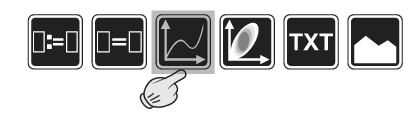
\includegraphics[width=0.45\textwidth]{graphics/how_to_use_fig8.png} \end{tabular}\end{center}

Plot panel with six empty fields
appears. The function to be plot shall
be put in the middle-left field and
the function argument in the
middle-bottom field:
\begin{center}\begin{tabular}{c} 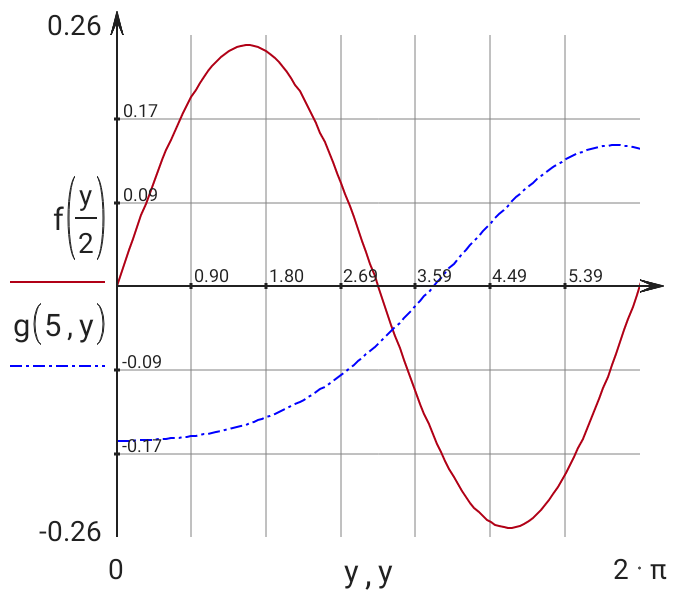
\includegraphics[width=0.45\textwidth]{graphics/how_to_use_fig9.png} \end{tabular}\end{center}

For more details see ''Function Plot''
and ''Polar Function Plot'' examples
from the app navigation drawer.

\subsection{Three-dimensional Plot}

The 3D plot element displays a graph of
a single function that depends on two
arguments. To create such a plot, use
the ''New element'' button in the action
bar or the ''Add 3D plot'' button from
the tool bar:
\begin{center}\begin{tabular}{c} 
\includegraphics[width=0.45\textwidth]{graphics/how_to_use_fig10.png} \end{tabular}\end{center}
\begin{center}\begin{tabular}{cc}
  $x := \left[ -10,\, -9.5 \,..\, 10 \right]$ &
  $y := \left[ -10,\, -9.5 \,..\, 10 \right]$ \cr
\end{tabular}\end{center}
\begin{center}\begin{tabular}{c} 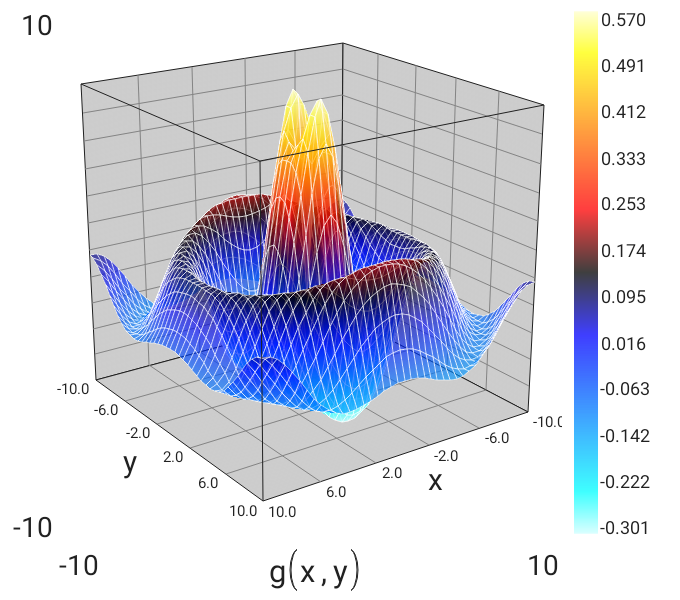
\includegraphics[width=0.45\textwidth]{graphics/how_to_use_fig11.png} \end{tabular}\end{center}

In the center-bottom field, put the
function name or an equation that
contains exactly two previously
defined intervals. The use of an array
is also possible:
\begin{center}\begin{tabular}{c} 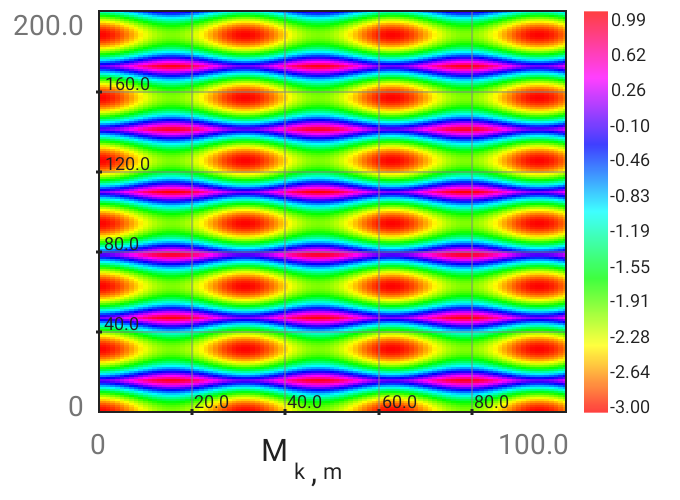
\includegraphics[width=0.45\textwidth]{graphics/how_to_use_fig12.png} \end{tabular}\end{center}

For more details see ''3D Plot'' example
from the app navigation drawer.

\subsection{Text Fragment}

The text fragment element displays
simple text like this one. To add a
text fragment, use the ''New element''
button in the action bar or ''Add text
fragment'' button from the tool bar:
\begin{center}\begin{tabular}{c} 
\includegraphics[width=0.45\textwidth]{graphics/how_to_use_fig13.png} \end{tabular}\end{center}

If the whole text within a fragment is 
selected using the context menu
''Select all'', a floating button
''Object properties'' appears in the
bottom-right of the screen.

If you click on this button, the ''Text
properties'' dialog will be displayed,
where you can select the text style
and activate the numbering. For
example, the titles in this document
have the style ''Subsection'' with
activated numbering.

\subsection{Image}

You can also insert an image from the
image file. To do it, use the ''New
element'' button from the action bar or
the ''Add image from file'' button from
the tool bar:
\begin{center}\begin{tabular}{c} 
\includegraphics[width=0.45\textwidth]{graphics/how_to_use_fig14.png} \end{tabular}\end{center}

The ''Image settings'' dialog will
appear. There you can select a file
with the image to be inserted and set
the necessary image size.

The following image formats are
supported: png, bmp, gif, jpeg, svg.

If you activate the ''Embedded image''
flag in the ''Image settings'' dialog,
then the image will be embedded
directly in your document. Embedded
image results in stand-alone, but
larger document.

If the ''Embedded image'' flag is not
set, the image file will be just
referenced rather than embedded, i.e.
your document references the image
file outside the document. In case you
move your document please do not
forget to move the image file as well.

You can change the properties of an
already existing image. Long click on
the image area until the floating
button ''Object properties'' appears. If
you press this button, a dialog with
image properties will be displayed.
